\chapter{Meiosis, mezcla genética y herencia}\label{ch:b2:meiosis-heredity}

Dos padres de ojos castaños tienen un hijo de ojos azules, y nadie se
sorprende; dos hijos de los mismos padres nunca son iguales, y tampoco
sorprende a nadie. Ambos hechos se derivan de un mismo proceso. En la
formación de cada óvulo y de cada espermatozoide, una célula con dos
copias de cada cromosoma transmite exactamente una, elegida al azar,
tras dejar que las dos copias intercambien segmentos. Cada fecundación
reúne después dos de esas mitades que nunca se habían encontrado. Este
capítulo describe ese proceso --- la \omterm{def:b2:meiosis-heredity:meiosis}{meiosis} --- y las reglas de la
herencia que se derivan de él: las proporciones de Mendel y sus
excepciones, el \omterm{def:b2:meiosis-heredity:linkage}{ligamiento} de los genes que comparten cromosoma y los
mapas que dibuja ese \omterm{def:b2:meiosis-heredity:linkage}{ligamiento}, y la herencia peculiar de los
\omterm{prop:b2:meiosis-heredity:sexlinked}{cromosomas sexuales} y de los orgánulos.

\section{La meiosis}

\begin{definition}[Meiosis]\label{def:b2:meiosis-heredity:meiosis}
\index{meiosis}\index{haploide}\index{diploide}
Una célula \emph{diploide} ($2n$) lleva dos cromosomas \emph{homólogos} de
cada tipo, uno de cada progenitor, iguales en contenido génico pero no
necesariamente en \omterm{def:b2:meiosis-heredity:vocabulary}{alelos}. La \emph{meiosis} es el par de divisiones que
convierte una célula diploide en cuatro células \emph{haploides} ($n$),
cada una con un cromosoma de cada tipo. La precede una única replicación,
de modo que cada cromosoma entra en ella con dos cromátidas hermanas; la
primera división separa los \emph{homólogos} (reduccional) y la segunda
separa las \emph{cromátidas hermanas} (ecuacional), como hace la mitosis.
En los animales la meiosis produce gametos; en las plantas y los hongos
produce esporas (\cref{ch:b2:plant-life-cycles}); en todo organismo con
reproducción sexual es la etapa que reduce a la mitad el número de
cromosomas para que la fecundación pueda volver a duplicarlo.
\end{definition}

\begin{proposition}[Las fases]\label{prop:b2:meiosis-heredity:stages}
\index{profase I}\index{sinapsis cromosómica}\index{quiasma}\index{entrecruzamiento}
La \emph{\omterm{prop:b2:meiosis-heredity:stages}{profase I}} es larga y es donde se produce la mezcla. Los
cromosomas replicados se condensan; cada uno encuentra a su homólogo y
se aparea con él gen a gen (\emph{sinapsis}), sujeto por una escalera
proteica, el \emph{complejo sinaptonémico}, para formar un
\emph{bivalente} de cuatro cromátidas; cromátidas no hermanas se rompen y
se vuelven a unir en puntos correspondientes (\emph{entrecruzamiento}),
una o varias veces por bivalente; cuando el complejo se disuelve, los
homólogos solo permanecen unidos por esos puntos de intercambio, visibles
como \emph{quiasmas}. \emph{Metafase I}: los bivalentes se alinean en el
huso, cada par orientado al azar --- el homólogo materno hacia un polo o
hacia el otro, con independencia de todos los demás pares.
\emph{Anafase I}: los homólogos se separan y las cromátidas hermanas
permanecen juntas; cada polo recibe $n$ cromosomas de dos cromátidas
cada uno. \emph{Telofase I} y, normalmente sin replicación,
\emph{\omterm{def:b2:meiosis-heredity:meiosis}{meiosis} II}: los $n$ cromosomas se alinean de uno en uno, las
cromátidas hermanas se separan y resultan cuatro núcleos \omterm{def:b2:meiosis-heredity:meiosis}{haploides}. La
\omterm{def:b2:meiosis-heredity:meiosis}{meiosis} I dura de horas a décadas (un ovocito humano queda detenido en
\omterm{prop:b2:meiosis-heredity:stages}{profase I} desde antes del nacimiento hasta la ovulación); la \omterm{def:b2:meiosis-heredity:meiosis}{meiosis} II
dura una hora.
\end{proposition}

\begin{omfigure}
\begin{tikzpicture}[every node/.style={font=\scriptsize}]
  % helper: cell outline at (x,y)
  \foreach \x/\lab in {0/{profase I: apareamiento, entrecruzamiento}, 3.2/{metafase I: bivalentes alineados}, 6.4/{anafase I: los homólogos se separan}, 9.6/{meiosis II: las cromátidas se separan}}
    { \draw[thick] (\x+1.2,0) circle (1.15); \node[below, align=center, text width=2.8cm] at (\x+1.2,-1.2) {\lab}; }
  % prophase I: one bivalent with chiasma
  \draw[very thick, omDef] (0.8,-0.5) -- (0.8,0.5); \draw[very thick, omDef] (1.0,-0.5) -- (1.0,0.5);
  \draw[very thick, omThm] (1.4,-0.5) -- (1.4,0.5); \draw[very thick, omThm] (1.6,-0.5) -- (1.6,0.5);
  \draw[very thick, omDef] (1.0,0.1) -- (1.4,-0.1); \draw[very thick, omThm] (1.4,0.1) -- (1.0,-0.1);
  \fill[white] (0.9,-0.03) rectangle (1.5,0.03);
  \draw[very thick, omDef] (1.0,0.1) -- (1.4,-0.1); \draw[very thick, omThm] (1.4,0.1) -- (1.0,-0.1);
  \node[omExo!60!black] at (1.2,-0.85) {quiasma};
  % metaphase I: two bivalents on the plate, spindle
  \begin{scope}[xshift=3.2cm]
    \draw[gray, dashed] (1.2,-1.0) -- (1.2,1.0);
    \foreach \y in {0.45,-0.45} {
      \draw[very thick, omDef] (0.95,\y-0.25) -- (0.95,\y+0.25); \draw[very thick, omDef] (1.08,\y-0.25) -- (1.08,\y+0.25);
      \draw[very thick, omThm] (1.32,\y-0.25) -- (1.32,\y+0.25); \draw[very thick, omThm] (1.45,\y-0.25) -- (1.45,\y+0.25);
    }
    \draw[gray] (0.15,0) -- (0.95,0.45); \draw[gray] (0.15,0) -- (0.95,-0.45);
    \draw[gray] (2.25,0) -- (1.45,0.45); \draw[gray] (2.25,0) -- (1.45,-0.45);
  \end{scope}
  % anaphase I
  \begin{scope}[xshift=6.4cm]
    \foreach \y in {0.45,-0.45} {
      \draw[very thick, omDef] (0.45,\y-0.25) -- (0.45,\y+0.25); \draw[very thick, omDef] (0.58,\y-0.25) -- (0.58,\y+0.25);
      \draw[very thick, omThm] (1.82,\y-0.25) -- (1.82,\y+0.25); \draw[very thick, omThm] (1.95,\y-0.25) -- (1.95,\y+0.25);
    }
    \draw[->, gray] (1.2,0) -- (0.75,0); \draw[->, gray] (1.2,0) -- (1.65,0);
  \end{scope}
  % meiosis II: four cells
  \begin{scope}[xshift=9.6cm]
    \foreach \p/\c in {(0.75,0.5)/omDef,(1.65,0.5)/omDef,(0.75,-0.5)/omThm,(1.65,-0.5)/omThm} {
      \draw[thick, gray!60] \p circle (0.38);
      \draw[very thick, \c] \p ++(-0.12,-0.2) -- ++(0,0.4);
      \draw[very thick, \c] \p ++(0.12,-0.2) -- ++(0,0.4);
    }
  \end{scope}
\end{tikzpicture}

{\small La \omterm{def:b2:meiosis-heredity:meiosis}{meiosis} para dos pares de homólogos (maternos en azul, paternos
en rojo, cada uno de dos cromátidas). Los homólogos se aparean e
intercambian segmentos en la \omterm{prop:b2:meiosis-heredity:stages}{profase I}, se alinean como bivalentes en la
metafase I y se separan en la anafase I; la \omterm{def:b2:meiosis-heredity:meiosis}{meiosis} II separa las
cromátidas en cuatro células \omterm{def:b2:meiosis-heredity:meiosis}{haploides}.}
\end{omfigure}

\begin{omfigure}
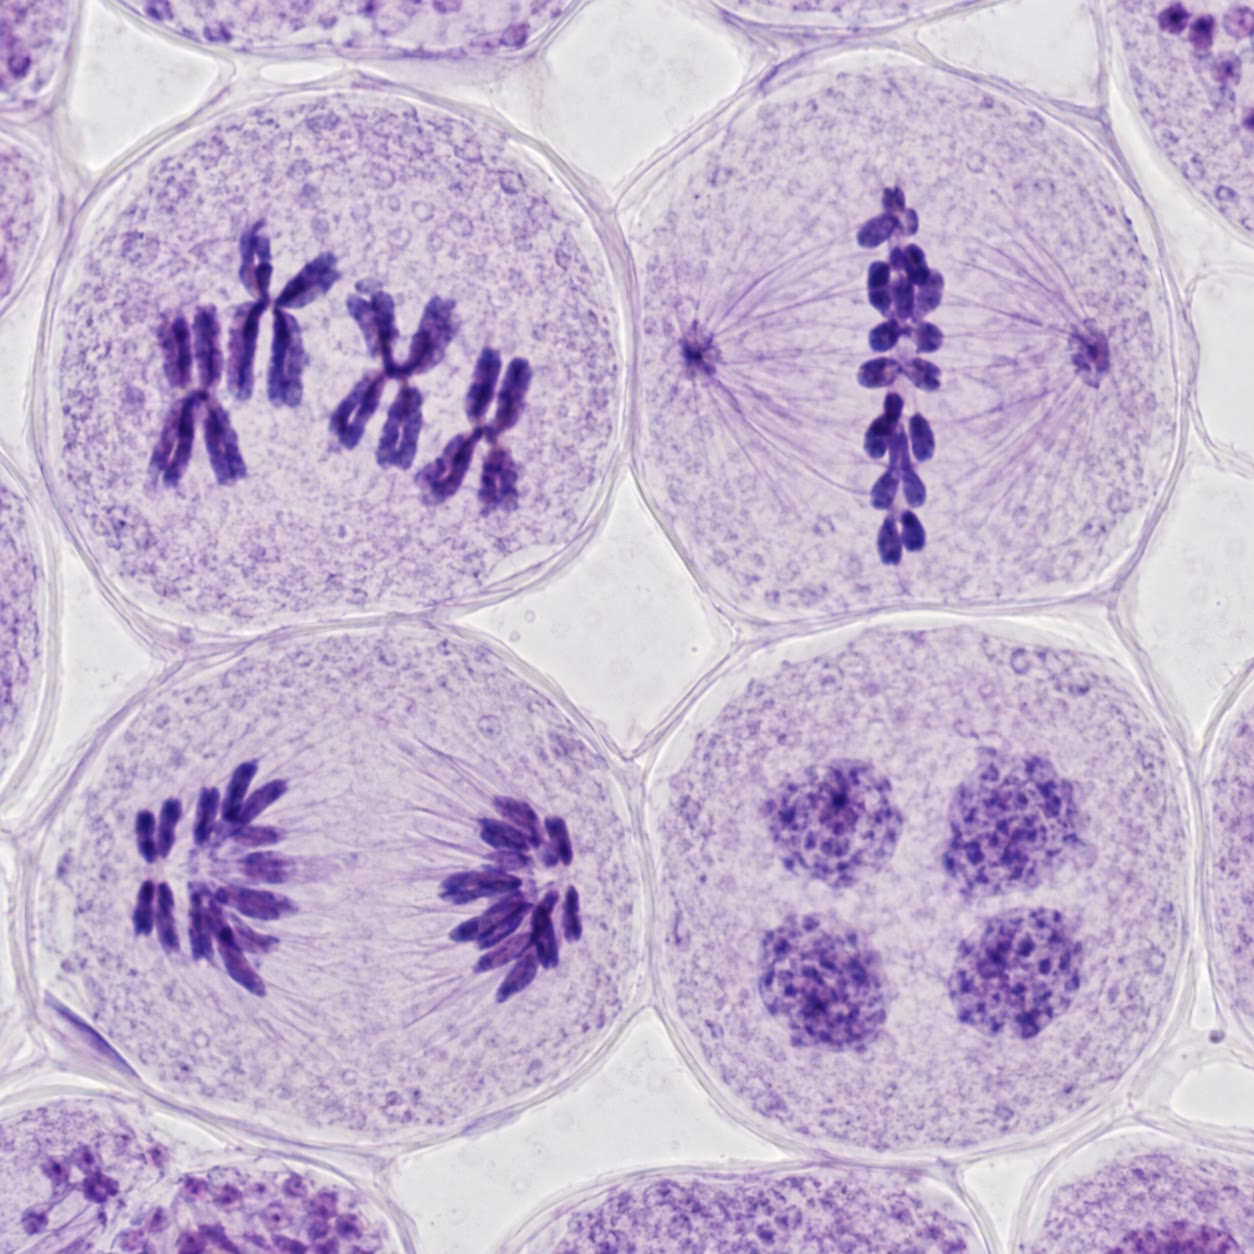
\includegraphics[width=0.5\linewidth]{images/book4/ai/b4-04-lily-meiosis.jpg}

{\small \omterm{def:b2:meiosis-heredity:meiosis}{Meiosis} en la antera de un lirio: bivalentes al final de la
\omterm{prop:b2:meiosis-heredity:stages}{profase I}, una placa de metafase I, la anafase I y los cuatro núcleos de
una tétrada.}
\end{omfigure}

\begin{theorem}[Cuánta mezcla produce la meiosis]\label{thm:b2:meiosis-heredity:mixing}
\index{segregación independiente}\index{recombinación genética}
En un organismo con $n$ pares de cromosomas, la orientación aleatoria de
los bivalentes en la metafase I produce $2^n$ combinaciones posibles de
cromosomas maternos y paternos en un gameto ---
$2^{23} \approx 8.4$ millones en el ser humano --- y $2^{2n}$ en un
cigoto. El entrecruzamiento multiplica esa cifra: con unos $k$ quiasmas
por bivalente, cada uno en una posición variable, el número de gametos
distintos es en la práctica ilimitado, y nunca dos gametos de una misma
persona son iguales. La \emph{recombinación} --- las nuevas combinaciones
de \omterm{def:b2:meiosis-heredity:vocabulary}{alelos} --- procede de ambos mecanismos: la \omterm{thm:b2:meiosis-heredity:mixing}{segregación independiente}
baraja cromosomas enteros; el entrecruzamiento baraja genes dentro de un
cromosoma.
\end{theorem}
\begin{proof}
Cada bivalente se orienta de forma independiente con dos resultados
posibles, de modo que $n$ bivalentes dan $2^n$ combinaciones, todas
igualmente probables. Cada uno de los dos progenitores aporta uno de esos
gametos, de modo que el cigoto tiene $2^n\times
2^n$. Un entrecruzamiento en una posición concreta de un cromosoma de $L$
pares de bases puede producir del orden de $L$ cromátidas recombinantes
distintas por bivalente, de modo que el número de productos distintos
crece como $L^k$ por cromosoma, lo que es astronómico para $L \sim 10^8$.
\end{proof}
\begin{proof}[Evidencia]
Creighton y McClintock (1931) usaron un cromosoma 9 de maíz que llevaba
dos marcas citológicas visibles (un botón en un extremo, un segmento
translocado en el otro) y, entre ellas, dos genes (grano coloreado o
incoloro, endospermo céreo o amiláceo). Entre los descendientes, toda
planta con un par de \omterm{def:b2:meiosis-heredity:vocabulary}{alelos} recombinado tenía también un par de marcas
citológicas recombinado --- botón sin translocación o a la inversa ---,
lo que demostró que la \omterm{thm:b2:meiosis-heredity:mixing}{recombinación genética} es un intercambio físico de
segmentos de cromosoma.
\end{proof}

\begin{omfigure}
\begin{tikzpicture}[every node/.style={font=\scriptsize}]
  \foreach \dx/\lab/\ca/\cb/\gam in {0/{orientación 1}/omDef/omThm/{gametos AB y ab}, 6.2/{orientación 2}/omThm/omDef/{gametos Ab y aB}} {
    \begin{scope}[xshift=\dx cm]
      \draw[gray, dashed] (0,-1.1) -- (3.2,-1.1);
      \node[anchor=south] at (1.6,0.6) {\lab};
      % pair 1 (long): A above the plate, a below
      \draw[very thick, omDef] (0.7,-0.95) -- (0.7,-0.25); \node[omDef, anchor=south] at (0.7,-0.2) {A};
      \draw[very thick, omThm] (0.7,-1.25) -- (0.7,-1.95); \node[omThm, anchor=north] at (0.7,-2.0) {a};
      % pair 2 (short): B or b above depending on orientation
      \draw[very thick, \ca] (2.3,-0.85) -- (2.3,-0.35);
      \draw[very thick, \cb] (2.3,-1.35) -- (2.3,-1.85);
      \node[anchor=north] at (1.6,-2.4) {\gam};
    \end{scope}
  }
  \node[omDef, anchor=south] at (2.3,-0.3) {B}; \node[omThm, anchor=north] at (2.3,-1.9) {b};
  \node[omThm, anchor=south] at (8.5,-0.3) {b}; \node[omDef, anchor=north] at (8.5,-1.9) {B};
  \node[anchor=north, align=center] at (4.7,-3.0) {cada orientación igual de probable:\\gametos AB, ab, Ab y aB en igual número --- segregación independiente};
\end{tikzpicture}

{\small \omterm{thm:b2:meiosis-heredity:mixing}{Segregación independiente}. Para dos pares de cromosomas (A/a en
uno, B/b en el otro), las dos orientaciones posibles de los bivalentes en
la metafase I son igual de probables, de modo que las cuatro
combinaciones de \omterm{def:b2:meiosis-heredity:vocabulary}{alelos} aparecen en igual número entre los gametos.}
\end{omfigure}

\section{El análisis mendeliano}

\begin{definition}[El vocabulario de los cruzamientos]\label{def:b2:meiosis-heredity:vocabulary}
\index{alelo}\index{genotipo}\index{fenotipo}\index{dominante}\index{recesivo}\index{homocigoto}\index{heterocigoto}
Un \emph{gen} es un tramo de cromosoma; sus \emph{alelos} son sus
variantes de secuencia; el \emph{locus} es su posición. Un individuo
\omterm{def:b2:meiosis-heredity:meiosis}{diploide} lleva dos alelos en cada locus: su \emph{genotipo}
es \emph{homocigoto} ($AA$, $aa$) o \emph{heterocigoto} ($Aa$).
El \emph{fenotipo} es el carácter observable. Un alelo es
\emph{dominante} cuando el heterocigoto muestra su fenotipo, y
\emph{recesivo} cuando solo se manifiesta en el homocigoto; la
distinción es una propiedad del par de alelos y del carácter observado,
no del alelo aislado --- la mayoría de los alelos recesivos son alelos
de pérdida de función, ocultos porque basta con una copia funcional. Una
\emph{línea pura} se reproduce sin variación (homocigota); un
\emph{cruzamiento de prueba} cruza un individuo de fenotipo dominante con
un homocigoto recesivo, de modo que su descendencia revela directamente
los alelos de sus gametos.
\end{definition}

\begin{theorem}[Las proporciones de Mendel]\label{thm:b2:meiosis-heredity:mendel}
\index{leyes de Mendel}\index{cruzamiento monohíbrido}\index{cruzamiento dihíbrido}
Como los dos \omterm{def:b2:meiosis-heredity:vocabulary}{alelos} de un \omterm{def:b2:meiosis-heredity:vocabulary}{heterocigoto} $Aa$ se reparten en gametos
distintos en igual número (anafase I), un cruzamiento \emph{monohíbrido}
$Aa \times Aa$ da los \omterm{def:b2:meiosis-heredity:vocabulary}{genotipos} $\tfrac14 AA : \tfrac12 Aa :
\tfrac14 aa$, y los \omterm{def:b2:meiosis-heredity:vocabulary}{fenotipos} $3 : 1$ si $A$ es \omterm{def:b2:meiosis-heredity:vocabulary}{dominante}; el cruzamiento
de prueba $Aa \times aa$ da $1 : 1$. Como los \omterm{def:b2:meiosis-heredity:vocabulary}{alelos} de genes situados
en cromosomas distintos se reparten de forma independiente (metafase I),
un \emph{dihíbrido} $AaBb$ produce cuatro tipos de gameto en igual número,
y el cruzamiento
$AaBb \times AaBb$ da los \omterm{def:b2:meiosis-heredity:vocabulary}{fenotipos} $9 : 3 : 3 : 1$, mientras que el
cruzamiento de prueba $AaBb \times aabb$ da $1 : 1 : 1 : 1$. Para $k$
loci \omterm{def:b2:meiosis-heredity:vocabulary}{heterocigotos} independientes, el número de tipos de gameto es $2^k$
y la proporción fenotípica es el producto de $k$ proporciones $3 : 1$.
\end{theorem}
\begin{proof}
Segregación: los gametos del \omterm{def:b2:meiosis-heredity:vocabulary}{heterocigoto} son $\tfrac12 A$,
$\tfrac12 a$; con fecundación al azar, los \omterm{def:b2:meiosis-heredity:vocabulary}{genotipos} del cigoto son los
productos $(\tfrac12 A + \tfrac12 a)^2 = \tfrac14 AA + \tfrac12 Aa +
\tfrac14 aa$. Independencia: los gametos de $AaBb$ son $(\tfrac12 A
+ \tfrac12 a)(\tfrac12 B + \tfrac12 b)$, cuatro tipos a $\tfrac14$;
los \omterm{def:b2:meiosis-heredity:vocabulary}{fenotipos} del dihíbrido multiplican $(\tfrac34 A\_ + \tfrac14 aa)
(\tfrac34 B\_ + \tfrac14 bb)$, lo que da $\tfrac{9}{16}, \tfrac{3}{16},
\tfrac{3}{16}, \tfrac{1}{16}$. Cada factor es una \omterm{thm:b2:meiosis-heredity:mixing}{segregación
independiente}, de modo que $k$ loci dan un producto de $k$ factores.
\end{proof}
\begin{proof}[Evidencia]
Mendel (1866) cruzó líneas puras de guisante que diferían en un carácter
--- semilla lisa o rugosa, cotiledón amarillo o verde, flor púrpura o
blanca, tallo alto o enano, y otros tres --- y encontró en todos los
casos una primera generación uniforme y una segunda generación que
segregaba cerca de $3 : 1$: 5474 lisas frente a 1850 rugosas ($2.96 :
1$), 6022 amarillas frente a 2001 verdes ($3.01 : 1$), 705 púrpuras frente
a 224 blancas
($3.15 : 1$). En los cruzamientos de dos caracteres encontró $315 : 108 : 101 :
32$ ($9 : 3 : 3 : 1$) y, cultivando la segunda generación, mostró que la
clase \omterm{def:b2:meiosis-heredity:vocabulary}{dominante} era de dos tipos, un tercio pura y dos tercios
segregantes. Los cromosomas que explican las proporciones se
descubrieron cuarenta años después.
\end{proof}

\begin{omfigure}
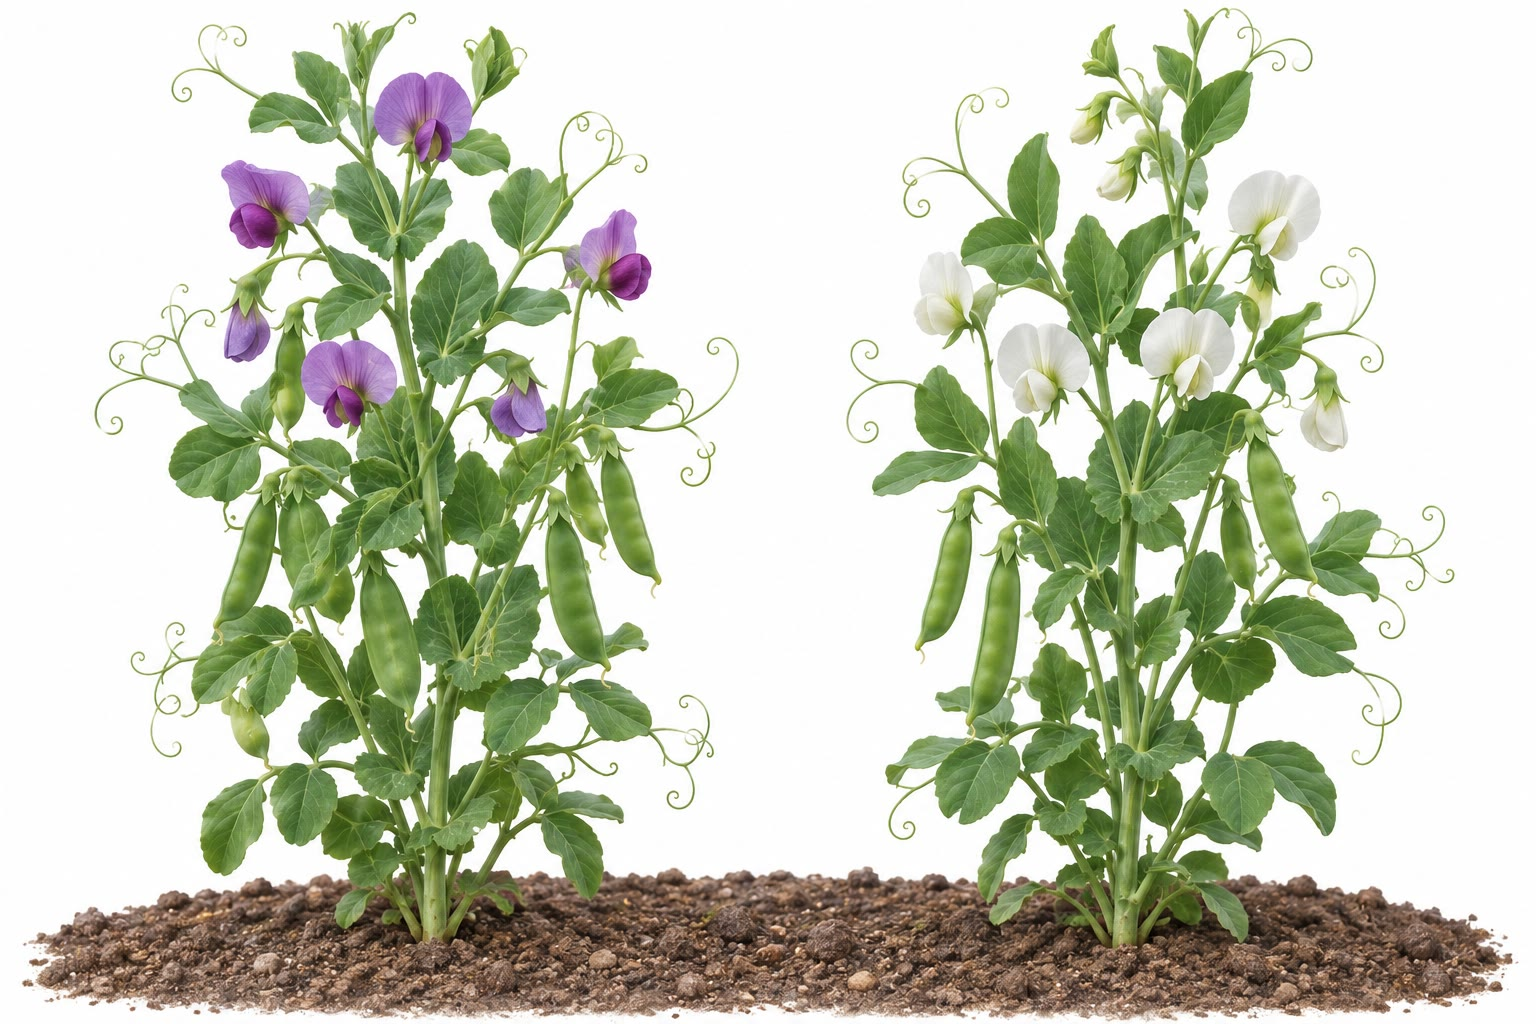
\includegraphics[width=0.58\linewidth]{images/book4/ai/b4-04-pea-flowers.jpg}

{\small Plantas de guisante de flor púrpura y de flor blanca: uno de los
siete pares de caracteres sobre los que Mendel fundó la genética. El
híbrido de flor púrpura, autofecundado, da unas tres púrpuras por cada
blanca.}
\end{omfigure}

\begin{method}[Contrastar una proporción con $\chi^2$]\label{met:b2:meiosis-heredity:chisquare}
\index{prueba de chi cuadrado}
Para decidir si unos recuentos observados $O_i$ se ajustan a una
proporción hipotética:
\begin{enumerate}
  \item Calcúlense los recuentos esperados $E_i$ a partir de la proporción
        y del total.
  \item Calcúlese $\chi^2 = \sum_i (O_i - E_i)^2/E_i$.
  \item Cuéntense los grados de libertad: el número de clases menos
        uno.
  \item Compárese con el valor crítico al nivel del \qty{5}{\%}:
        $3.84$ para 1 grado de libertad, $5.99$ para 2, $7.81$ para 3,
        $9.49$ para 4. Si $\chi^2$ queda por debajo, los datos son
        compatibles con la proporción; si queda por encima, la proporción
        se rechaza --- la desviación surgiría por azar en menos de un
        experimento de cada veinte.
\end{enumerate}
Para las flores de Mendel, $705 : 224$ frente a $3 : 1$: $E = 696.75,
232.25$; $\chi^2 = 0.098 + 0.293 = 0.39 < 3.84$. (La distribución en la
que se basan los valores críticos se deduce en la estadística de la
serie de matemáticas; aquí la tabla es una herramienta.)
\end{method}

\begin{proposition}[Más allá de las proporciones simples]\label{prop:b2:meiosis-heredity:extensions}
\index{dominancia incompleta}\index{codominancia}\index{epistasia}\index{alelo letal}
Las proporciones cambian, pero el mecanismo no, cuando: los \omterm{def:b2:meiosis-heredity:vocabulary}{alelos}
muestran \emph{\omterm{prop:b2:meiosis-heredity:extensions}{dominancia incompleta}} (una boca de dragón roja $\times$
blanca da rosa, y la segunda generación $1 : 2 : 1$); los \omterm{def:b2:meiosis-heredity:vocabulary}{alelos} son
\emph{codominantes}, ambos expresados (sangre $AB$: el \omterm{def:b2:meiosis-heredity:vocabulary}{heterocigoto}
$I^AI^B$ fabrica los dos antígenos; un locus puede tener \emph{\omterm{def:b2:meiosis-heredity:vocabulary}{alelos}
múltiples}, $I^A$, $I^B$, $i$); un \omterm{def:b2:meiosis-heredity:vocabulary}{alelo} es \emph{letal} en
homocigosis (ratones amarillos: amarillo $\times$ amarillo da $2$
amarillos por
$1$ agutí, pues el $\tfrac14 YY$ muere en estado embrionario); dos genes
actúan en una misma ruta (\emph{epistasia}: en un cruzamiento
$9 : 3 : 3 : 1$ el doble \omterm{def:b2:meiosis-heredity:vocabulary}{recesivo} y uno de los \omterm{def:b2:meiosis-heredity:vocabulary}{recesivos} simples pueden
ser indistinguibles, lo que da
$9 : 3 : 4$, como en los ratones albinos, o pueden hacer falta los dos
\omterm{def:b2:meiosis-heredity:vocabulary}{dominantes} para el \omterm{def:b2:meiosis-heredity:vocabulary}{fenotipo}, lo que da $9 : 7$, como en los guisantes de
olor púrpuras, que necesitan dos enzimas para fabricar su pigmento);
muchos genes suman cada uno un poco a un carácter continuo (altura,
rendimiento), lo que constituye la genética cuantitativa del
\cref{ch:b2:population-genetics}. Remontarse de una proporción a un
mecanismo es el oficio cotidiano de la genética.
\end{proposition}

\section{Ligamiento y mapas genéticos}

\begin{definition}[Ligamiento y frecuencia de recombinación]\label{def:b2:meiosis-heredity:linkage}
\index{ligamiento}\index{frecuencia de recombinación}\index{centimorgan}
Dos genes situados en el mismo cromosoma están \emph{ligados}: sus \omterm{def:b2:meiosis-heredity:vocabulary}{alelos}
tienden a viajar juntos a los gametos, y un dihíbrido
$AB/ab$ produce más gametos \emph{parentales} ($AB$, $ab$) que
\emph{recombinantes} ($Ab$, $aB$). Los recombinantes solo aparecen cuando
un entrecruzamiento cae entre los dos loci, de modo que su frecuencia
$r$ --- contada directamente en un cruzamiento de prueba --- mide la
distancia: $r$ va de 0 (ligamiento completo) a $\tfrac12$ (genes tan
alejados, o en cromosomas distintos, que se reparten de forma
independiente). La unidad de \emph{distancia genética} es el
\emph{centimorgan} (cM): \qty{1}{cM} equivale a un \qty{1}{\%} de
recombinación para genes estrechamente ligados; en el ser humano,
\qty{1}{cM} corresponde a alrededor de un millón de pares de bases. El
ligamiento fue la primera prueba de que los genes están dispuestos en
línea a lo largo del cromosoma.
\end{definition}
\begin{proof}[Evidencia]
Morgan (1911) observó que los genes de ojo blanco y de ala miniatura de la
mosca, ambos en el cromosoma X, no se repartían de forma independiente:
un cruzamiento de prueba daba un \qty{37}{\%} de recombinantes en lugar
de un \qty{50}{\%}, y otros pares daban otros porcentajes, reproducibles.
Sturtevant (1913), todavía estudiante, comprendió que si las frecuencias
miden distancias deben sumarse: a partir de las frecuencias por pares de
seis genes ligados al X dibujó el primer mapa genético, y las distancias
eran, dentro del error, aditivas a lo largo de una línea.
\end{proof}

\begin{omfigure}
\begin{tikzpicture}[every node/.style={font=\scriptsize}]
  % bivalent with crossover between A and B
  \draw[very thick, omDef] (0,1.2) -- (2.0,1.2) -- (3.0,0.6) -- (5,0.6);
  \draw[very thick, omDef] (0,1.5) -- (5,1.5);
  \draw[very thick, omThm] (0,0.3) -- (2.0,0.3) -- (3.0,0.9) -- (5,0.9);
  \draw[very thick, omThm] (0,0) -- (5,0);
  \node[omDef, above] at (0.8,1.5) {A}; \node[omDef, above] at (4.3,1.5) {B};
  \node[omThm, below] at (0.8,0) {a}; \node[omThm, below] at (4.3,0) {b};
  \node[anchor=south, gray] at (2.5,1.85) {entrecruzamiento entre los loci A y B};
  % products
  \draw[->, thick, gray] (5.4,0.75) -- (6.2,0.75);
  \node[anchor=west, align=left] at (6.4,1.45) {\textcolor{omDef}{A\,B} \quad parental};
  \node[anchor=west, align=left] at (6.4,0.95) {\textcolor{omDef}{A}\,\textcolor{omThm}{b} \quad recombinante};
  \node[anchor=west, align=left] at (6.4,0.5) {\textcolor{omThm}{a}\,\textcolor{omDef}{B} \quad recombinante};
  \node[anchor=west, align=left] at (6.4,0.0) {\textcolor{omThm}{a\,b} \quad parental};
  \node[anchor=west, align=left, text width=5.6cm] at (6.4,-0.9) {un entrecruzamiento entre los loci en una fracción $c$ de las meiosis: gametos recombinantes $r = c/2$, porque solo se intercambian dos de las cuatro cromátidas};
\end{tikzpicture}

{\small Recombinación entre dos loci ligados. Un entrecruzamiento entre
ellos en un bivalente intercambia los \omterm{def:b2:meiosis-heredity:vocabulary}{alelos} de dos de las cuatro
cromátidas; los gametos recombinantes se cuentan en un cruzamiento de
prueba, y su frecuencia mide la distancia.}
\end{omfigure}

\begin{method}[Cartografiar dos genes ligados]\label{met:b2:meiosis-heredity:twopoint}
\begin{enumerate}
  \item Crúcense dos líneas puras para obtener el dihíbrido; anótese qué
        \omterm{def:b2:meiosis-heredity:vocabulary}{alelos} recibió juntos (sus combinaciones parentales, en
        \emph{acoplamiento} $AB/ab$ o en \emph{repulsión} $Ab/aB$).
  \item Hágase un cruzamiento de prueba con el doble \omterm{def:b2:meiosis-heredity:vocabulary}{recesivo} y
        clasifíquense los descendientes: las dos clases más numerosas son
        las parentales, las dos menos numerosas las recombinantes.
  \item $r = $ recombinantes $/$ total; la distancia es $100\,r$ cM.
  \item Compruébese antes la independencia: si las cuatro clases son
        iguales ($\chi^2$ frente a $1 : 1 : 1 : 1$), los genes no están
        ligados.
\end{enumerate}
\end{method}

\begin{theorem}[La función cartográfica de Haldane]\label{thm:b2:meiosis-heredity:haldane}
\index{función cartográfica}
La \omterm{def:b2:meiosis-heredity:linkage}{frecuencia de recombinación} subestima la distancia entre genes muy
alejados, porque dos entrecruzamientos entre ellos restablecen la
combinación parental. Si los entrecruzamientos caen de forma
independiente a lo largo del cromosoma (sin interferencia), con $d$ la
distancia genética en morgans (número esperado de entrecruzamientos por
cromátida), la fracción de recombinación es
\[
r = \tfrac12\,\bigl(1 - e^{-2d}\bigr), \qquad d = -\tfrac12\ln(1 - 2r),
\]
de modo que $r \approx d$ para $d$ pequeña y $r \to \tfrac12$ cuando $d$
crece; $r = 0.40$ corresponde a \qty{80}{cM}, y \qty{50}{cM}
dan $r = 0.32$. Los cromosomas reales muestran \emph{interferencia} ---
un entrecruzamiento hace menos probable otro cercano ---, lo que acerca
$r$ a $d$ más de lo que predice Haldane en distancias cortas.
\end{theorem}
\begin{proof}
Sea la distancia genética $d$ el número esperado de entrecruzamientos por
cromátida en el intervalo; como todo entrecruzamiento implica a dos de
las cuatro cromátidas, el bivalente en su conjunto lleva en el intervalo
un número de entrecruzamientos que sigue una ley de Poisson de media
$2d$, y la probabilidad de que no lleve ninguno es $e^{-2d}$. Si lleva al
menos uno, cada entrecruzamiento implica de forma independiente a una
cromátida dada con probabilidad
$\tfrac12$, de modo que una cromátida dada ha sido intercambiada un
número impar de veces --- es recombinante --- con probabilidad
exactamente $\tfrac12$, cualquiera que sea el número de
entrecruzamientos. Por tanto $r = \tfrac12\,(1 -
e^{-2d})$; invirtiendo se obtiene $d$. Para $d$ pequeña, $r \approx d$;
cuando $d \to \infty$, $r \to \tfrac12$.
\end{proof}
\begin{omfigure}
\begin{tikzpicture}
\begin{axis}[
  width=0.72\linewidth, height=5.6cm,
  axis x line=bottom, axis y line=left,
  xmin=0, xmax=150, ymin=0, ymax=0.55,
  xlabel={distancia genética $d$ (cM)}, ylabel={fracción de recombinación $r$},
  xlabel style={font=\small, at={(axis description cs:0.5,-0.13)}, anchor=north},
  ylabel style={font=\small},
  tick label style={font=\small}, xtick={0,50,100,150}, ytick={0,0.25,0.5},
  legend style={font=\scriptsize, at={(0.97,0.1)}, anchor=south east, draw=none},
  clip=false,
]
\addplot[very thick, omDef, domain=0:150, samples=80] {0.5*(1-exp(-2*x/100))};
\addlegendentry{Haldane: $r = \tfrac12(1 - e^{-2d})$}
\addplot[thick, dashed, gray, domain=0:50, samples=2] {x/100};
\addlegendentry{$r = d$ (sin dobles entrecruzamientos)}
\draw[dashed, gray] (axis cs:0,0.5) -- (axis cs:150,0.5);
\end{axis}
\end{tikzpicture}

{\small Fracción de recombinación en función de la distancia genética.
Los genes cercanos recombinan en proporción a su distancia; los genes
lejanos nunca superan el \qty{50}{\%} de recombinación, por alejados que
estén, porque los dobles entrecruzamientos restablecen las combinaciones
parentales.}
\end{omfigure}

\begin{method}[El cruzamiento de prueba de tres puntos]\label{met:b2:meiosis-heredity:threepoint}
\index{cruzamiento de tres puntos}\index{interferencia}
Crúcese un triple \omterm{def:b2:meiosis-heredity:vocabulary}{heterocigoto} $ABC/abc$ con $abc/abc$ y clasifíquense
las ocho clases de descendientes.
\begin{enumerate}
  \item Las dos clases más grandes son las parentales; las dos más
        pequeñas son los \emph{dobles entrecruzamientos}.
  \item El gen que cambia entre una clase parental y la clase de doble
        entrecruzamiento es el \emph{central}: eso da el orden.
  \item Para cada par adyacente, la \omterm{def:b2:meiosis-heredity:linkage}{frecuencia de recombinación} es
        (entrecruzamientos simples en ese intervalo + dobles
        entrecruzamientos) $/$ total, puesto que un doble
        entrecruzamiento recombina ambos intervalos.
  \item Dobles entrecruzamientos esperados $= r_1 r_2 \times$ total; el
        \emph{coeficiente de coincidencia} es observados/esperados, y la
        \emph{interferencia} es $1 -$ coincidencia.
\end{enumerate}
\end{method}

\begin{example}[Un cruzamiento de tres puntos resuelto]\label{ex:b2:meiosis-heredity:threepoint}
Descendientes de $+++/abc \times abc/abc$: $+++$ 580, $abc$ 592, $++c$
45, $ab+$ 40, $+bc$ 89, $a++$ 94, $+b+$ 3, $a+c$ 5; total 1448.
Parentales $+++$, $abc$; dobles $+b+$, $a+c$; comparando $+++$ con
$+b+$, el gen que ha cambiado es $b$: orden $a$--$b$--$c$. $r_{ab} =
(89 + 94 + 3 + 5)/1448 = 0.132$; $r_{bc} = (45 + 40 + 3 + 5)/1448 =
0.064$; mapa: $a$ --- \qty{13.2}{cM} --- $b$ --- \qty{6.4}{cM} ---
$c$. Dobles esperados $0.132\times 0.064\times 1448 = 12.2$,
observados 8: coincidencia $0.65$, interferencia $0.35$.
\end{example}

\begin{omfigure}
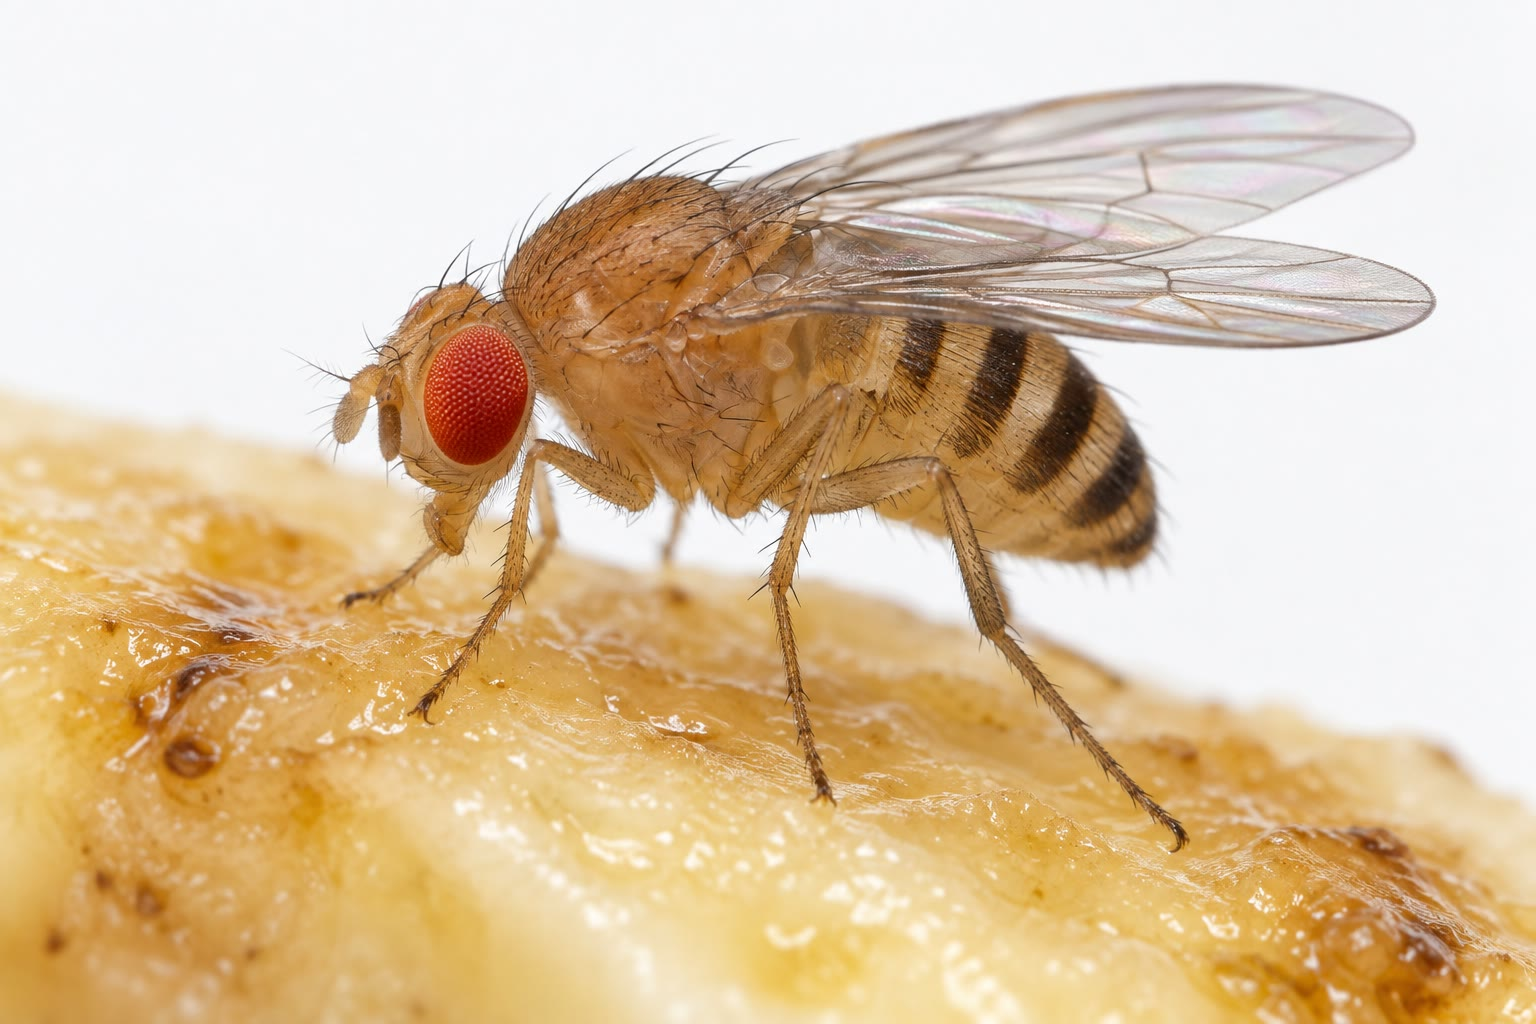
\includegraphics[width=0.5\linewidth]{images/book4/ai/b4-04-drosophila.jpg}

{\small \emph{Drosophila melanogaster}: dos semanas por generación,
cientos de descendientes, cuatro pares de cromosomas y un siglo de
mutantes --- el organismo con el que se descifraron el \omterm{def:b2:meiosis-heredity:linkage}{ligamiento}, los
mapas y la herencia ligada al sexo.}
\end{omfigure}

\section{Cromosomas sexuales y orgánulos}

\begin{proposition}[Herencia ligada al sexo]\label{prop:b2:meiosis-heredity:sexlinked}
\index{herencia ligada al X}\index{cromosomas sexuales}
En los mamíferos y las moscas la hembra es $XX$ y el macho $XY$: el $Y$
lleva pocos genes, de modo que un macho tiene una sola copia de cada gen
ligado al $X$ (es \emph{hemicigoto}) y manifiesta el \omterm{def:b2:meiosis-heredity:vocabulary}{alelo} que lleve,
sea \omterm{def:b2:meiosis-heredity:vocabulary}{dominante} o \omterm{def:b2:meiosis-heredity:vocabulary}{recesivo}. Consecuencias: los cruzamientos recíprocos
difieren (hembra de ojos blancos $\times$ macho de ojos rojos da hijos de
ojos blancos e
hijas de ojos rojos; el cruzamiento inverso da todos rojos); un carácter
\omterm{def:b2:meiosis-heredity:vocabulary}{recesivo} ligado al
$X$ (daltonismo rojo--verde, hemofilia, distrofia muscular de
Duchenne) aparece sobre todo en los varones, lo transmiten madres
portadoras no afectadas y nunca pasa de padre a hijo (un hijo recibe el
$Y$ de su padre); un padre transmite su $X$ a todas sus hijas.
Las aves, las mariposas y algunos reptiles invierten la disposición
(hembras $ZW$, machos $ZZ$); en muchos reptiles decide la temperatura; y
en los mamíferos uno de los $X$ de cada célula femenina se silencia al
azar al comienzo del desarrollo, de modo que una hembra heterocigota es
un mosaico (la gata carey).
\end{proposition}
\begin{proof}[Evidencia]
Morgan (1910) encontró un macho de ojos blancos entre miles de moscas de
ojos rojos. Cruzado con hembras rojas, toda la descendencia fue roja;
pero en la generación siguiente los ojos blancos reaparecieron solo en
los machos, en la mitad de ellos. Cruzar un macho blanco con sus hijas
rojas dio ojos blancos en ambos sexos. El patrón era exactamente el
esperado si el gen estaba en el cromosoma X, que las hembras llevan dos
veces y los machos una --- el primer gen asignado a un cromosoma.
\end{proof}

\begin{omfigure}
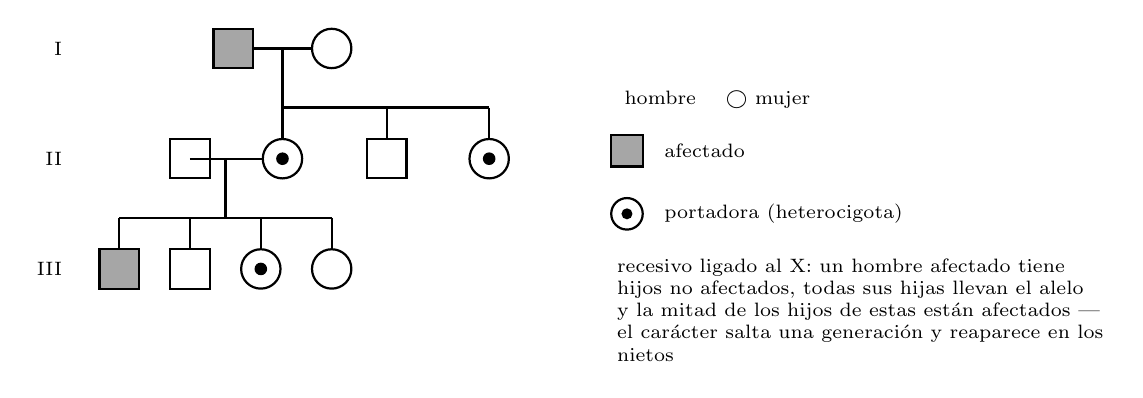
\begin{tikzpicture}[every node/.style={font=\scriptsize}]
  % pedigree: X-linked recessive
  \draw[thick, fill=gray!70] (0,0) rectangle (0.5,0.5); % affected grandfather
  \draw[thick] (1.5,0.25) circle (0.25);
  \draw[thick] (0.5,0.25) -- (1.25,0.25);
  \draw[thick] (0.875,0.25) -- (0.875,-0.5);
  \draw[thick] (0.875,-0.5) -- (3.5,-0.5);
  % children of generation I
  \draw[thick] (0.875,-0.5) -- (0.875,-0.9); \draw[thick, fill=white] (0.875,-1.15) circle (0.25); \fill (0.875,-1.15) circle (0.08);
  \draw[thick] (2.2,-0.5) -- (2.2,-0.9); \draw[thick] (1.95,-1.4) rectangle (2.45,-0.9);
  \draw[thick] (3.5,-0.5) -- (3.5,-0.9); \draw[thick, fill=white] (3.5,-1.15) circle (0.25); \fill (3.5,-1.15) circle (0.08);
  % carrier daughter marries
  \draw[thick] (-0.3,-1.15) -- (0.625,-1.15); \draw[thick] (-0.55,-1.4) rectangle (-0.05,-0.9);
  \draw[thick] (0.15,-1.15) -- (0.15,-1.9); \draw[thick] (-1.2,-1.9) -- (1.5,-1.9);
  \draw[thick] (-1.2,-1.9) -- (-1.2,-2.3); \draw[thick, fill=gray!70] (-1.45,-2.8) rectangle (-0.95,-2.3);
  \draw[thick] (-0.3,-1.9) -- (-0.3,-2.3); \draw[thick] (-0.55,-2.8) rectangle (-0.05,-2.3);
  \draw[thick] (0.6,-1.9) -- (0.6,-2.3); \draw[thick, fill=white] (0.6,-2.55) circle (0.25); \fill (0.6,-2.55) circle (0.08);
  \draw[thick] (1.5,-1.9) -- (1.5,-2.3); \draw[thick, fill=white] (1.5,-2.55) circle (0.25);
  \node[anchor=east] at (-1.8,0.25) {I};
  \node[anchor=east] at (-1.8,-1.15) {II};
  \node[anchor=east] at (-1.8,-2.55) {III};
  % legend
  \node[anchor=west, align=left] at (5,-0.4) {$\square$ hombre \quad $\bigcirc$ mujer};
  \draw[thick, fill=gray!70] (5.05,-1.25) rectangle (5.45,-0.85); \node[anchor=west] at (5.6,-1.05) {afectado};
  \draw[thick] (5.25,-1.85) circle (0.2); \fill (5.25,-1.85) circle (0.07); \node[anchor=west] at (5.6,-1.85) {portadora (heterocigota)};
  \node[anchor=north west, align=left, text width=6.2cm] at (5,-2.3) {recesivo ligado al X: un hombre afectado tiene hijos no afectados, todas sus hijas llevan el alelo y la mitad de los hijos de estas están afectados --- el carácter salta una generación y reaparece en los nietos};
\end{tikzpicture}

{\small \omterm{met:b2:meiosis-heredity:pedigree}{Árbol genealógico} de un carácter \omterm{def:b2:meiosis-heredity:vocabulary}{recesivo} ligado al X, como la
hemofilia: sin transmisión de padre a hijo, hijas portadoras, nietos
afectados.}
\end{omfigure}

\begin{method}[Leer un árbol genealógico]\label{met:b2:meiosis-heredity:pedigree}
\index{árbol genealógico}
\begin{enumerate}
  \item Dos padres no afectados con un hijo afectado: el carácter es
        \omterm{def:b2:meiosis-heredity:vocabulary}{recesivo} (ambos progenitores \omterm{def:b2:meiosis-heredity:vocabulary}{heterocigotos}).
  \item Un hijo afectado tiene siempre un progenitor afectado, y el
        carácter aparece en todas las generaciones: \omterm{def:b2:meiosis-heredity:vocabulary}{dominante}.
  \item Afectados sobre todo varones, transmisión a través de madres no
        afectadas, nunca de padre a hijo: \omterm{def:b2:meiosis-heredity:vocabulary}{recesivo} ligado al X.
  \item Un padre afectado tiene todas sus hijas afectadas y ningún hijo
        afectado: \omterm{def:b2:meiosis-heredity:vocabulary}{dominante} ligado al X.
  \item Transmitido por las madres a todos sus hijos, nunca por los
        padres: mitocondrial.
  \item Calcúlense después las probabilidades a partir de los \omterm{def:b2:meiosis-heredity:vocabulary}{genotipos}
        implicados: una pareja portadora $\times$ normal tiene en cada
        nacimiento una probabilidad de $\tfrac14$ de tener un hijo varón
        afectado ($\tfrac12$ varón $\times$ $\tfrac12$ recibe el \omterm{def:b2:meiosis-heredity:vocabulary}{alelo}).
\end{enumerate}
\end{method}

\begin{definition}[Herencia extranuclear]\label{def:b2:meiosis-heredity:extranuclear}
\index{herencia materna}\index{herencia mitocondrial}
Las mitocondrias y los cloroplastos llevan sus propios genomas pequeños,
en muchas copias por orgánulo y muchos orgánulos por célula, y proceden
casi por completo del óvulo: el espermatozoide aporta un núcleo y poco
más. Sus genes son, por tanto, de \emph{herencia
materna}, sin proporciones de segregación: una madre transmite el
carácter a todos sus hijos; un padre, a ninguno. Las enfermedades
mitocondriales humanas (defectos de la cadena respiratoria que afectan al
músculo y al nervio) siguen este patrón, y también el variegado de
algunas plantas, en las que una célula madre que contiene cloroplastos
normales y mutantes los reparte al azar entre sus células hijas, lo que
produce sectores verdes, blancos y mixtos. Como nunca recombinan, las
secuencias mitocondriales permiten remontar los linajes maternos en el
tiempo --- la herramienta del \cref{ch:b2:phylogenetic-trees}.
\end{definition}

\begin{proposition}[Análisis de tétradas]\label{prop:b2:meiosis-heredity:tetrads}
\index{análisis de tétradas}\index{tétrada ordenada}
En algunos hongos (\emph{Neurospora}, \emph{Sordaria}) los cuatro
productos de una \omterm{def:b2:meiosis-heredity:meiosis}{meiosis} permanecen juntos en un saco, el \emph{asco}, y
en orden: una mitosis final da ocho esporas cuya secuencia registra las
dos divisiones. Para un \omterm{def:b2:meiosis-heredity:vocabulary}{heterocigoto} $A/a$, un asco con el patrón
$4 : 4$ (\emph{segregación en la primera división}) no tuvo ningún
entrecruzamiento entre el gen y su centrómero --- los \omterm{def:b2:meiosis-heredity:vocabulary}{alelos} se separaron
en la anafase I; un
patrón $2 : 2 : 2 : 2$ o $2 : 4 : 2$ (\emph{segregación en la segunda
división}) tuvo uno, de modo que los \omterm{def:b2:meiosis-heredity:vocabulary}{alelos} solo se separaron en la
anafase II. La distancia del gen al centrómero es la mitad del porcentaje
de ascos de segunda división, porque un entrecruzamiento solo recombina
dos de las cuatro cromátidas. Las tétradas muestran también directamente
que la recombinación es recíproca: toda cromátida recombinante tiene su
compañera complementaria en el mismo asco.
\end{proposition}

\begin{omfigure}
\begin{tikzpicture}[every node/.style={font=\scriptsize}]
  \foreach \dx/\pat/\lab in {0/{omDef,omDef,omDef,omDef,omThm,omThm,omThm,omThm}/{$4:4$, sin\\entrecruzamiento:\\segregación en la\\primera división}, 4.5/{omDef,omDef,omThm,omThm,omDef,omDef,omThm,omThm}/{$2:2:2:2$,\\entrecruzamiento entre\\el gen y el centrómero}, 9/{omDef,omDef,omThm,omThm,omThm,omThm,omDef,omDef}/{$2:4:2$,\\entrecruzamiento:\\segregación en la\\segunda división}} {
    \begin{scope}[xshift=\dx cm]
      \draw[thick, rounded corners=6pt] (0,0) rectangle (0.8,4.2);
      \foreach \c [count=\i] in \pat { \fill[\c] (0.4,4.2-0.5*\i+0.02) circle (0.2); }
      \node[below, align=center] at (0.4,-0.1) {\lab};
    \end{scope}
  }
  \node[anchor=west, align=left, text width=2.6cm] at (12.4,3.2) {ascos ordenados de \emph{Sordaria}; las esporas azules y rojas llevan los dos alelos};
\end{tikzpicture}

{\small \omterm{prop:b2:meiosis-heredity:tetrads}{Tétradas ordenadas}. Sin entrecruzamiento entre el gen y su
centrómero, los \omterm{def:b2:meiosis-heredity:vocabulary}{alelos} se separan en la primera división y las ocho
esporas se leen $4 : 4$; con uno, se separan en la segunda división y el
asco se lee $2 : 2 : 2 : 2$ o $2 : 4 : 2$.}
\end{omfigure}

\section{Ejercicios}

\begin{exercise}[$\star$]\label{exo:b2:meiosis-heredity:1}
Enumérense cuatro diferencias entre mitosis y \omterm{def:b2:meiosis-heredity:meiosis}{meiosis} (número de
divisiones, apareamiento, productos, identidad genética de los
productos).
\end{exercise}

\begin{exercise}[$\star$]\label{exo:b2:meiosis-heredity:2}
¿Cuántos gametos cromosómicamente distintos puede producir una persona
solo por \omterm{thm:b2:meiosis-heredity:mixing}{segregación independiente}? ¿Y una mosca del vinagre ($n = 4$)?
¿Y un guisante ($n =
7$)?
\end{exercise}

\begin{exercise}[$\star$]\label{exo:b2:meiosis-heredity:3}
En el guisante, el tallo alto ($T$) domina sobre el enano. Dense las
proporciones fenotípicas y genotípicas de $Tt \times Tt$ y de
$Tt \times tt$. ¿Cómo se averigua si una planta alta es $TT$ o $Tt$?
\end{exercise}

\begin{exercise}[$\star$]\label{exo:b2:meiosis-heredity:4}
Defínanse el \omterm{def:b2:meiosis-heredity:linkage}{ligamiento}, la \omterm{def:b2:meiosis-heredity:linkage}{frecuencia de recombinación} y el \omterm{def:b2:meiosis-heredity:linkage}{centimorgan}.
¿Por qué dos genes del mismo cromosoma pueden, pese a todo, repartirse
como si fueran independientes?
\end{exercise}

\begin{exercise}[$\star\star$]\label{exo:b2:meiosis-heredity:5}
El \omterm{thm:b2:meiosis-heredity:mendel}{cruzamiento dihíbrido} de Mendel dio $315$ lisas amarillas, $108$
lisas verdes, $101$ rugosas amarillas y $32$ rugosas verdes. Contrástese
la hipótesis $9 : 3 : 3 :
1$ con $\chi^2$ (3 grados de libertad, valor crítico
$7.81$).
\end{exercise}

\begin{exercise}[$\star\star$]\label{exo:b2:meiosis-heredity:6}
Un dihíbrido $AB/ab$ sometido a un cruzamiento de prueba da $412$ $AB$,
$388$ $ab$, $103$
$Ab$ y $97$ $aB$. ¿Están ligados los genes? Calcúlense la \omterm{def:b2:meiosis-heredity:linkage}{frecuencia de
recombinación} y la distancia genética; ¿qué daría el dihíbrido $Ab/aB$?
\end{exercise}

\begin{exercise}[$\star\star$]\label{exo:b2:meiosis-heredity:7}
Con la función de Haldane, conviértanse $r = 0.20$ y $r = 0.45$ en
distancias genéticas, y \qty{30}{cM} y \qty{100}{cM} en fracciones de
recombinación. Coméntese qué conversiones importan en la práctica.
\end{exercise}

\begin{exercise}[$\star\star$]\label{exo:b2:meiosis-heredity:8}
En \emph{Drosophila}, el ojo blanco ($w$) es \omterm{def:b2:meiosis-heredity:vocabulary}{recesivo} ligado al X. Dense
los descendientes, por sexo y \omterm{def:b2:meiosis-heredity:vocabulary}{fenotipo}, de (a) una hembra blanca $\times$
un macho rojo, (b) una hembra roja heterocigota $\times$ un macho blanco,
(c) el cruzamiento de las hijas de (a) con sus hermanos.
\end{exercise}

\begin{exercise}[$\star\star$]\label{exo:b2:meiosis-heredity:9}
Dos líneas puras de guisante de olor de flor blanca, cruzadas, dan una
descendencia toda púrpura, que autofecundada da $9$ púrpuras : $7$
blancas. Explíquese con dos genes, dense los \omterm{def:b2:meiosis-heredity:vocabulary}{genotipos} de las dos líneas
parentales y predígase el resultado de un cruzamiento de prueba del
híbrido púrpura.
\end{exercise}

\begin{exercise}[$\star\star\star$]\label{exo:b2:meiosis-heredity:10}
Un cruzamiento de prueba de tres puntos da: $+++$ 480, $abc$ 470, $+bc$ 11,
$a++$ 9, $++c$ 118, $ab+$ 112, $+b+$ 1, $a+c$ 1 (total 1202). Hállense
el orden de los genes, las dos distancias, el coeficiente de coincidencia
y la interferencia.
\end{exercise}

\begin{exercise}[$\star\star\star$]\label{exo:b2:meiosis-heredity:11}
En \emph{Sordaria}, un cruzamiento de una cepa de esporas negras con otra
de esporas pardas da $700$ ascos con patrón $4 : 4$ y $300$ con
patrones $2 : 2 : 2 : 2$ o $2 : 4 : 2$. Calcúlese la distancia del gen
del color de las esporas a su centrómero, y explíquese por qué hace
falta el factor un medio. Dibújense las cromátidas de una \omterm{def:b2:meiosis-heredity:meiosis}{meiosis} que dé
$2 : 4 : 2$.
\end{exercise}

\begin{exercise}[$\star\star\star$]\label{exo:b2:meiosis-heredity:12}
El abuelo materno de una mujer tenía hemofilia; nadie más en la familia
está afectado. ¿Cuál es la probabilidad de que ella sea portadora? Dado
que ha tenido dos hijos varones sanos, ¿cuál es ahora? Muéstrese el
razonamiento.
\end{exercise}

\section{Problema: cruzamientos en la sala de las moscas}

\begin{problem}[{Problema de fin de semana --- cruzamientos de
\emph{Drosophila} analizados desde la proporción monohíbrida hasta un
mapa de tres puntos, y un \omterm{met:b2:meiosis-heredity:pedigree}{árbol genealógico} humano calculado, hasta
llegar al mapa de tres genes ligados al X y a su interferencia}]
\label{pb:b2:meiosis-heredity:1}
Las alas vestigiales ($vg$) y el cuerpo ébano ($e$) son \omterm{def:b2:meiosis-heredity:vocabulary}{recesivos} y están
en autosomas distintos; el cuerpo negro ($b$) y $vg$ son \omterm{def:b2:meiosis-heredity:vocabulary}{recesivos} y
ambos están en el cromosoma 2; el cuerpo amarillo ($y$), el ojo blanco
($w$) y el ala miniatura ($m$) son \omterm{def:b2:meiosis-heredity:vocabulary}{recesivos} y están ligados al X.
Valores críticos de $\chi^2$ al
\qty{5}{\%}: $3.84$ (1 g.l.), $7.81$ (3 g.l.).

\medskip
\noindent\textbf{Parte I --- Dos genes autosómicos.}
Una mosca vestigial pura se cruza con una mosca ébano pura; la $F_1$ es
toda de tipo silvestre; se examinan $1600$ moscas $F_2$: $892$ silvestres,
$309$ vestigiales, $296$ ébano, $103$ vestigiales ébano.
\begin{enumerate}
  \item Dense los \omterm{def:b2:meiosis-heredity:vocabulary}{genotipos} de los progenitores, de la $F_1$ y de los
        gametos de la $F_1$.
  \item Calcúlense los recuentos esperados bajo \omterm{thm:b2:meiosis-heredity:mixing}{segregación independiente}.
  \item Calcúlese $\chi^2$ y conclúyase.
  \item ¿Qué fracción de las moscas $F_2$ de tipo silvestre es homocigota
        en ambos loci?
  \item Se hace un cruzamiento de prueba de la $F_1$ con una mosca
        vestigial ébano: predíganse las cuatro clases y sus proporciones.
  \item Las moscas ébano criadas a \qty{29}{\celsius} son más pálidas que
        a \qty{18}{\celsius}. ¿Qué dice esto de la relación entre
        \omterm{def:b2:meiosis-heredity:vocabulary}{genotipo} y \omterm{def:b2:meiosis-heredity:vocabulary}{fenotipo}?
\end{enumerate}

\medskip
\noindent\textbf{Parte II --- Dos genes ligados.}
Una mosca negra pura se cruza con una mosca vestigial pura; las hembras
$F_1$ se someten a un cruzamiento de prueba con machos negros
vestigiales: $965$ negras,
$944$ vestigiales, $206$ negras vestigiales, $185$ de tipo silvestre.
\begin{enumerate}[resume]
  \item Escríbase el \omterm{def:b2:meiosis-heredity:vocabulary}{genotipo} de la $F_1$, indicando qué \omterm{def:b2:meiosis-heredity:vocabulary}{alelos} están en
        el mismo cromosoma.
  \item Identifíquense las clases parentales y recombinantes, y
        explíquese por qué aquí el tipo silvestre es \emph{recombinante}.
  \item Calcúlense $r$ y la distancia genética.
  \item Corríjase con la función de Haldane.
  \item El mismo cruzamiento, con \emph{machos} $F_1$ en el cruzamiento de
        prueba, solo da dos clases, negras y vestigiales, en igual número.
        ¿Qué muestra esto sobre la \omterm{def:b2:meiosis-heredity:meiosis}{meiosis} en los machos de la mosca?
  \item Predíganse las clases y sus proporciones si la hembra $F_1$
        procediera de un cruzamiento negra vestigial $\times$ silvestre.
\end{enumerate}

\medskip
\noindent\textbf{Parte III --- Un \omterm{met:b2:meiosis-heredity:pedigree}{árbol genealógico} humano.}
La hemofilia A es recesiva ligada al X. Un hombre con hemofilia tiene una
hija, que se casa con un hombre no afectado.
\begin{enumerate}[resume]
  \item ¿Cuál es el \omterm{def:b2:meiosis-heredity:vocabulary}{genotipo} de la hija, y por qué es seguro?
  \item Probabilidad de que su primer hijo sea un varón afectado.
  \item Probabilidad de que una hija suya sea portadora.
  \item Probabilidad de que, entre sus tres hijos, ninguno esté
        afectado.
  \item Explíquese por qué la enfermedad nunca pasa de padre a hijo, y
        cómo podría estar afectada una mujer.
  \item La hermana del hombre afectado tiene dos hijos varones sanos; su
        madre (la madre del hombre) era portadora. Calcúlese la
        probabilidad de que la hermana sea portadora, antes y después de
        tener en cuenta a sus hijos.
\end{enumerate}

\medskip
\noindent\textbf{Parte IV --- Tres genes ligados al X.}
Una hembra $y\,w\,m/+\,+\,+$ se cruza con un macho $y\,w\,m$; se examinan
sus $2000$
hijos varones: $+++$ 853, $ywm$ 833, $y++$ 24, $+wm$ 26, $yw+$ 128,
$++m$ 132, $+w+$ 2, $y+m$ 2.
\begin{enumerate}[resume]
  \item ¿Por qué pueden examinarse directamente los hijos varones, sin
        cruzamiento de prueba?
  \item Identifíquense las clases parentales y de doble entrecruzamiento y
        dedúzcase el orden de los genes.
  \item Calcúlense las dos \omterm{def:b2:meiosis-heredity:linkage}{frecuencias de recombinación} y dibújese el mapa.
  \item Calcúlense el número esperado de dobles entrecruzamientos, el
        coeficiente de coincidencia y la interferencia.
  \item Calcúlese directamente a partir de los datos la \omterm{def:b2:meiosis-heredity:linkage}{frecuencia de
        recombinación} entre los dos genes externos, y explíquese por qué
        es menor que la suma de las dos distancias.
  \item ¿Cómo serían las hijas de este cruzamiento, y por qué no sirven
        para cartografiar?
  \item Enúnciese el resultado: el mapa de los tres genes y la
        interferencia.
\end{enumerate}
\end{problem}
